\chapter{Guiding Case Study: LaGuardia}
\label{ch:atrds}

This chapter will contain the primary technical contribution of the thesis. Here, we will perform a guiding case study that will serve as both a proof of concept and motivation for further directions of study, which will we begin to explore in \cref{app:atm}, \cref{app:risk}, and \cref{app:shrinkage}. It is also important to note that it is a simplified proof of concept that may seem over-complicated at first, for the simple scenario. However, this is done intentionally to show how we would develop more complex methods for this use case, which may be necessary background for future work such as moving our problem up from tabular weather data to weather image or video generation.

\section{Overview}

As a proof of concept for the general proposed study, we consider a simplified model of the relationship between weather and delays at LaGuardia Airport (LGA), and provide a demonstration of simultaneously inferring the posterior distribution of the latent parameters and fitting our model to historical data. We use stochastic variational inference (SVI), as introduced in \cref{background-variational-inference}, to learn an approximation for the posterior, and develop a simple form of amortized inference to demonstrate how it can be used for failure prediction and test case generation. 

\section{Single Airport Problem}
\label{sec:atrds-single-airport}
To motivate the decisions made in our simplified model, we first perform an initial analysis of our empirical data. We will be focusing on the mean service time as our latent variable $\rz$, which is inversely related to airport capacity, or maximum throughput of arrival and departure events, and work on the timescale of a full day for the granularity of $\rz$ and $\rw$, i.e. we only have a single value for each day. Here, we will be assuming that we have a fully specified model for the $\pld{x\given z;y}$ component, but still need to learn $\pld{z\given w}$, which we will do at the same time as learning the relevant posteriors.

\subsection{Flight Data}
Scheduled and actual flight times are taken from the Bureau of Transportation Statistics (BTS) Reporting Carrier On-Time Performance database \cite{bts_transstats_nodate}. Flights from the years 2018 and 2019 are used for training, but analysis is focused on July 2019. Specifically, for each flight in a day, we take the scheduled departure and arrival times for the context $y$, and the actual times for observations $x$, where times are converted to hours past midnight in LGA local time. We restrict our focus to modeling accumulated delays throughout the day, so we do not make additional provisions for cancellations or diversions.

Later, in \cref{sec:atrds-theory}, we will also need to use a coarser encoding of $x$ and $y$ on the same timescale as $z$ and $w$. For this, we will define our aggregation for $x$ as the straight average across all flights in the day, where flights that arrive early are considered as having zero delay instead of negative delay. We will aggregate $y$ by counting the number of operations scheduled in each hour of the day, and taking the maximum, as shown in \cref{fig:split-scheduled-capacity}. We also tried using the total number of flights in the day as a measure of aggregate scheduled demand, and obtained similar results.

\begin{figure}[htb!]
    \centering
    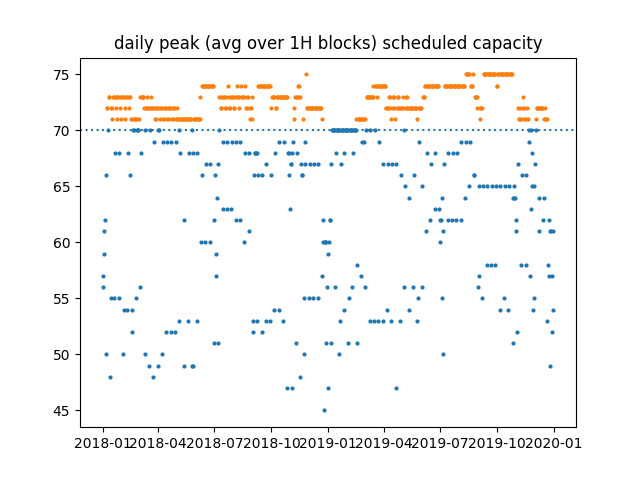
\includegraphics[width=0.8\linewidth]{media/lga-analysis-14.png}
    \caption{Daily peak scheduled hourly demand in 2018 and 2019, in operations per hour.}
    \label{fig:split-scheduled-capacity}
\end{figure}

\subsection{Weather Data}
We restrict our focus to considering the impact of visibility and ceiling, as these weather conditions are known to directly affect airport capacity \cite{2014lga}. Measurements are taken from the National Oceanic and Atmospheric Administration (NOAA) Local Climatological Data Version 2 (LCDv2) dataset \cite{weatherdata}, and converted to the Meteorological Aerodrome Report (METAR) format commonly used in aviation. Specifically, visibility is already given as an hourly value, but ceiling must be inferred from provided sky condition data by taking the height of the lowest cloud layer with at least 4 oktas of coverage.

For our encoding as a daily aggregate value, we use the harmonic mean~\cite{ferger1931nature} for the sky ceiling, to reflect the greater relevance of lower values, and similarly select the daily minimum for the visibility. We clip values at $10000$ feet and $10$ statute miles for ceiling and visibility respectively, for numerical stability, and because there is not really any meaningful difference among higher values.


\subsection{Initial Motivating Analysis}

To see why our choice of variables is well motivated for a proof of concept study, we examine the relationship between weather and delays, which our learned model should be able to reflect, if it is a good representation. First, we note that lower ceilings and visibilities appear to partially coincide with days with higher delays, as shown in \cref{fig:2019-07-weather-delay-timeline}.

\begin{figure}[htb!]
    \centering
    % 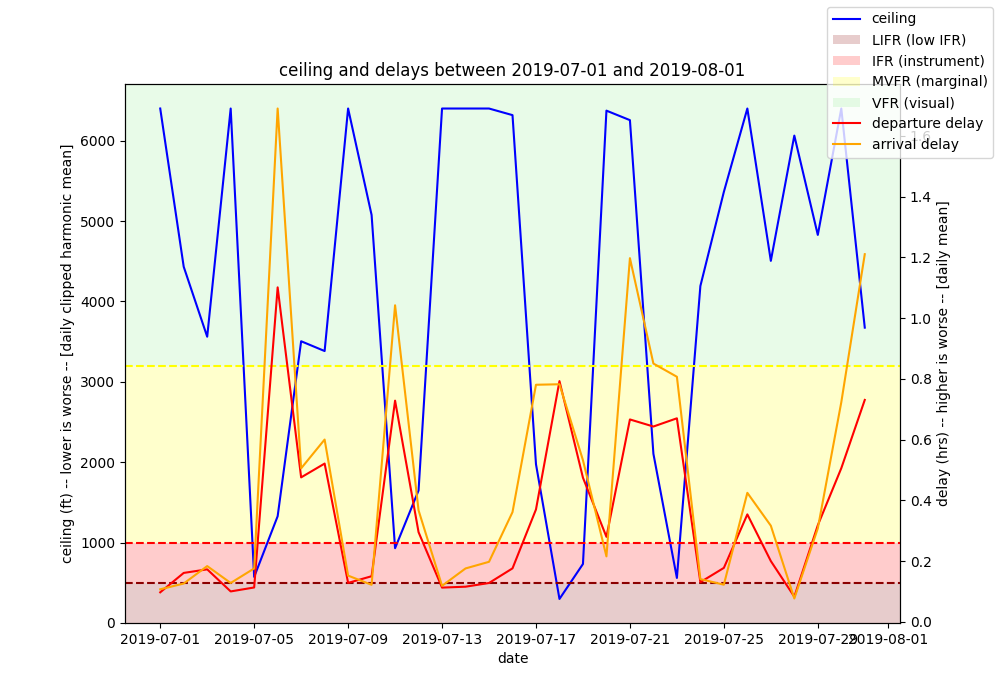
\includegraphics[height=5.5cm]{media/lga-analysis-1.png}
    % 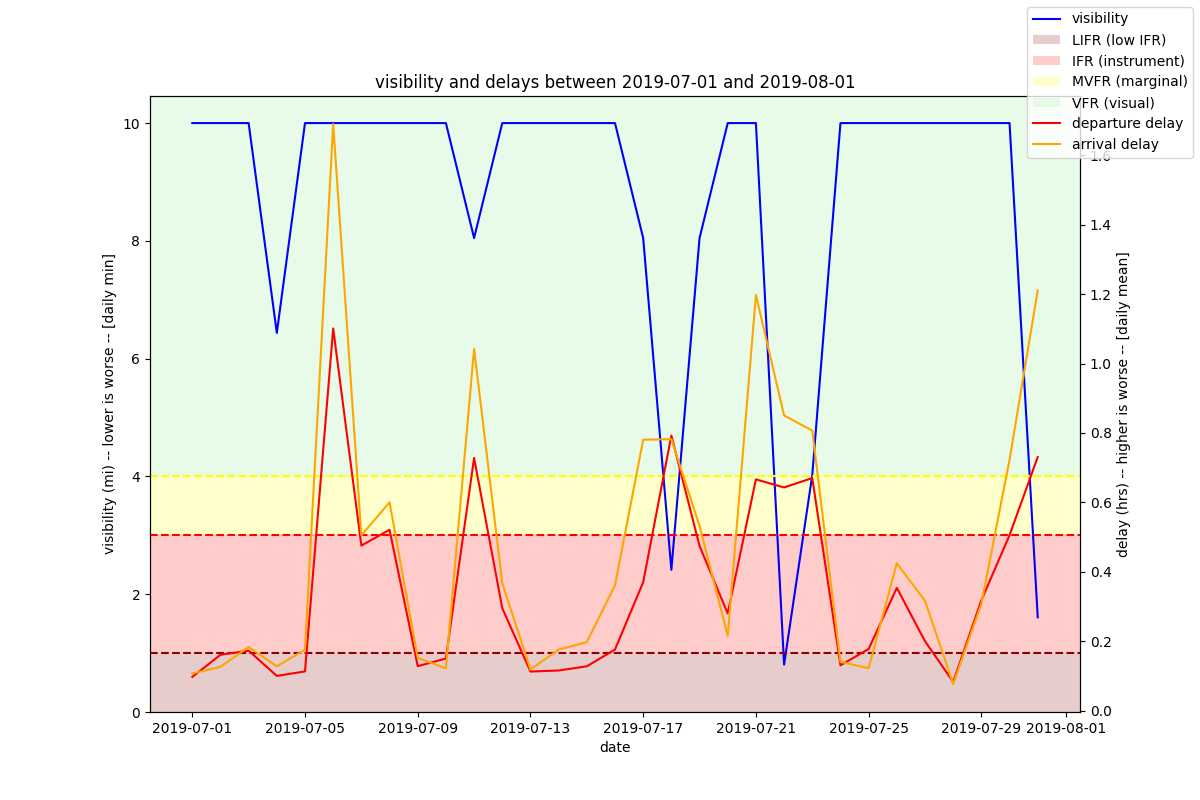
\includegraphics[height=5.5cm]{media/lga-analysis-3.png}
    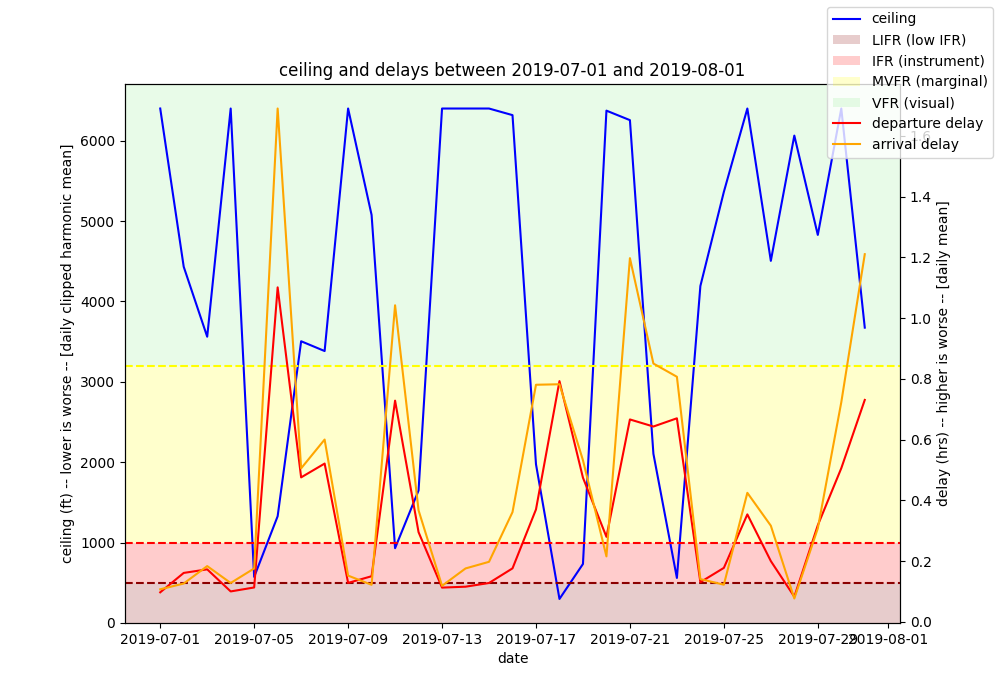
\includegraphics[width=.66\linewidth]{media/lga-analysis-1.png}
    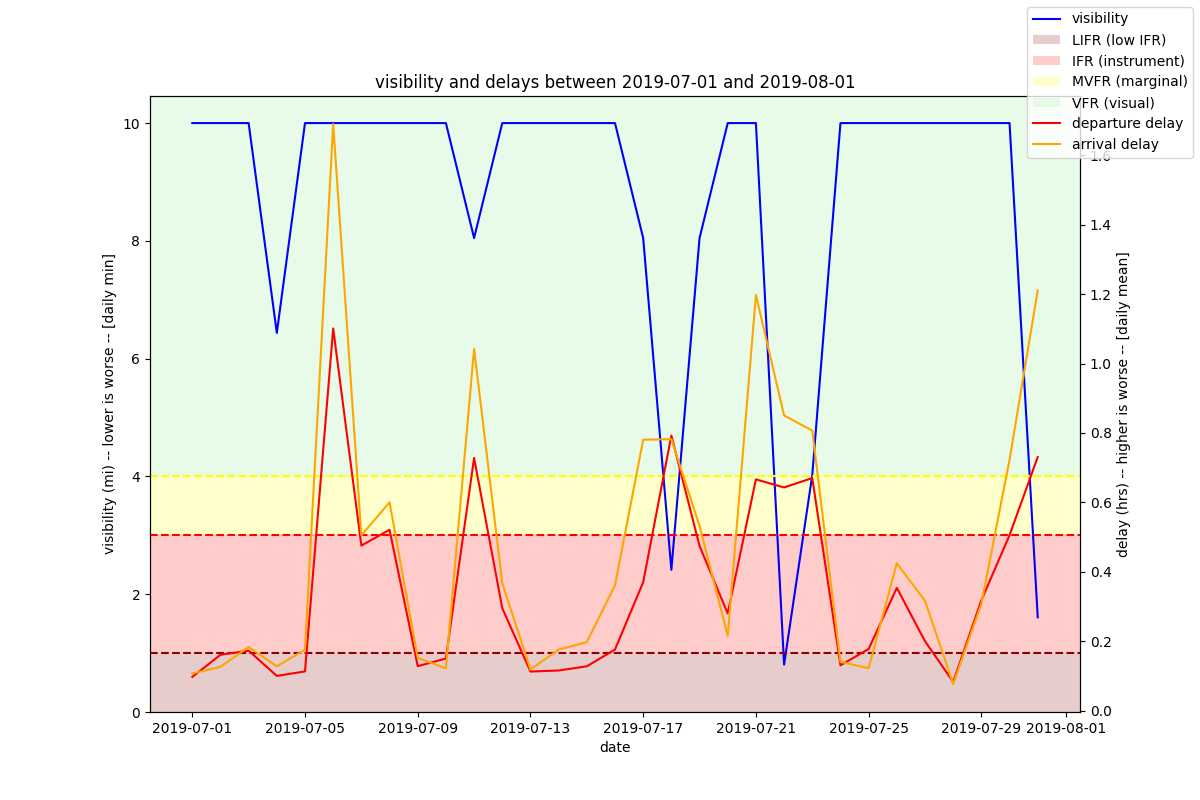
\includegraphics[width=.66\linewidth]{media/lga-analysis-3.png}
    \caption{Timeline of ceiling (upper) and visibility (lower) compared to delays in July 2019. Days with poorer weather, where the blue line is lower, coincide with days with greater delays, where the red and orange lines are higher. Flight rule regions show severity of weather.}
    \label{fig:2019-07-weather-delay-timeline}
\end{figure}

\begin{figure}[htb!]
    \centering
    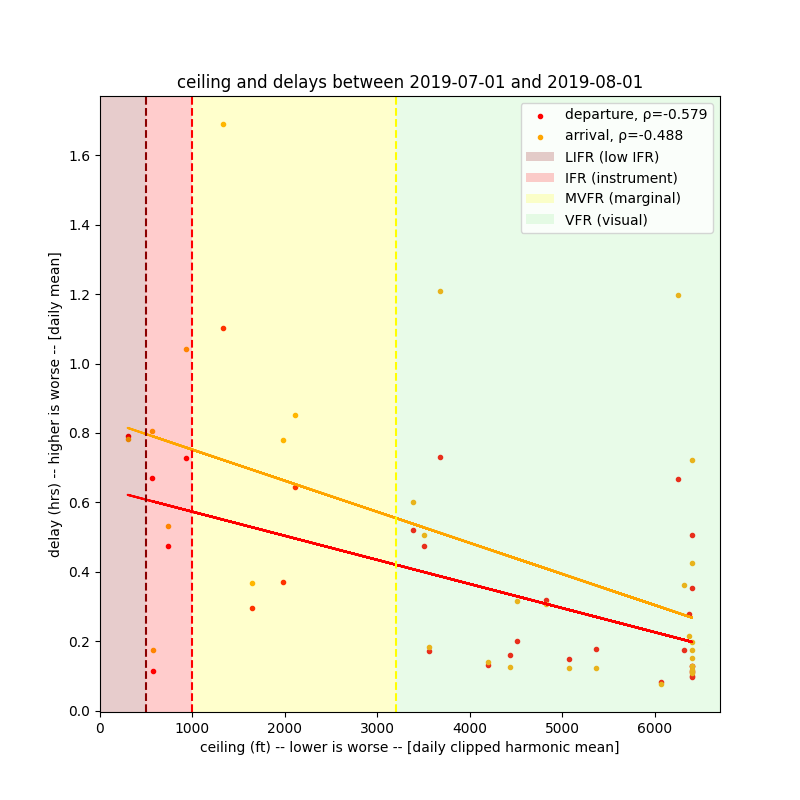
\includegraphics[height=8.1cm]{media/lga-analysis-2.png}
    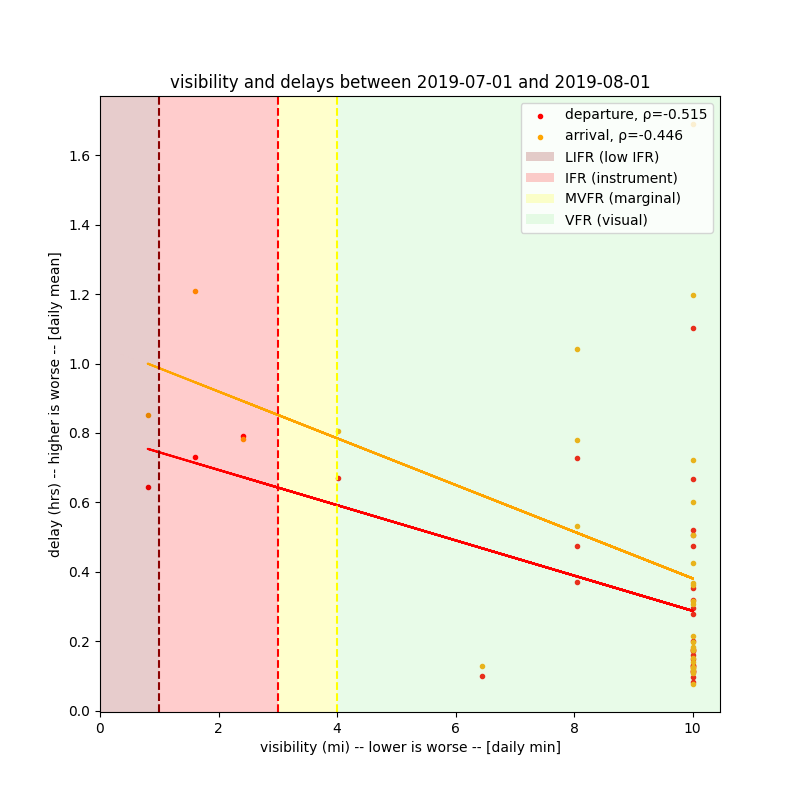
\includegraphics[height=8.1cm]{media/lga-analysis-4.png}
    \caption{Scatter plot of ceiling (left) and visibility (right) compared to delays in July 2019.}
    \label{fig:2019-07-weather-delay-scatter}
\end{figure}

Here, instrument flight rule (IFR) weather conditions are supposed to lead to a lower maximum throughput, meaning likely higher delays, than visual flight rule (VFR) conditions, which appears to align well with what we observe. To make this relationship a bit more obvious, we also show the same data in the timeline as a scatter plot with trend line and Pearson correlation coefficient, in \cref{fig:2019-07-weather-delay-scatter}. 


It is important to re-iterate, however, that weather is not the only factor that is considered in modeling delays, as is emphasized in \cref{fig:bubble3d-all}. We can see that higher scheduled capacity, corresponding to busier days, are more prone to delays at the same weather conditions compared to a lighter day, for example. This distinction in distribution of delays given weather is illustrated in \cref{fig:bubble2d-split}, which is essentially a 2D top view of an upper and lower partition of the full 3D plot.

\begin{figure}[htb!]
    \centering
    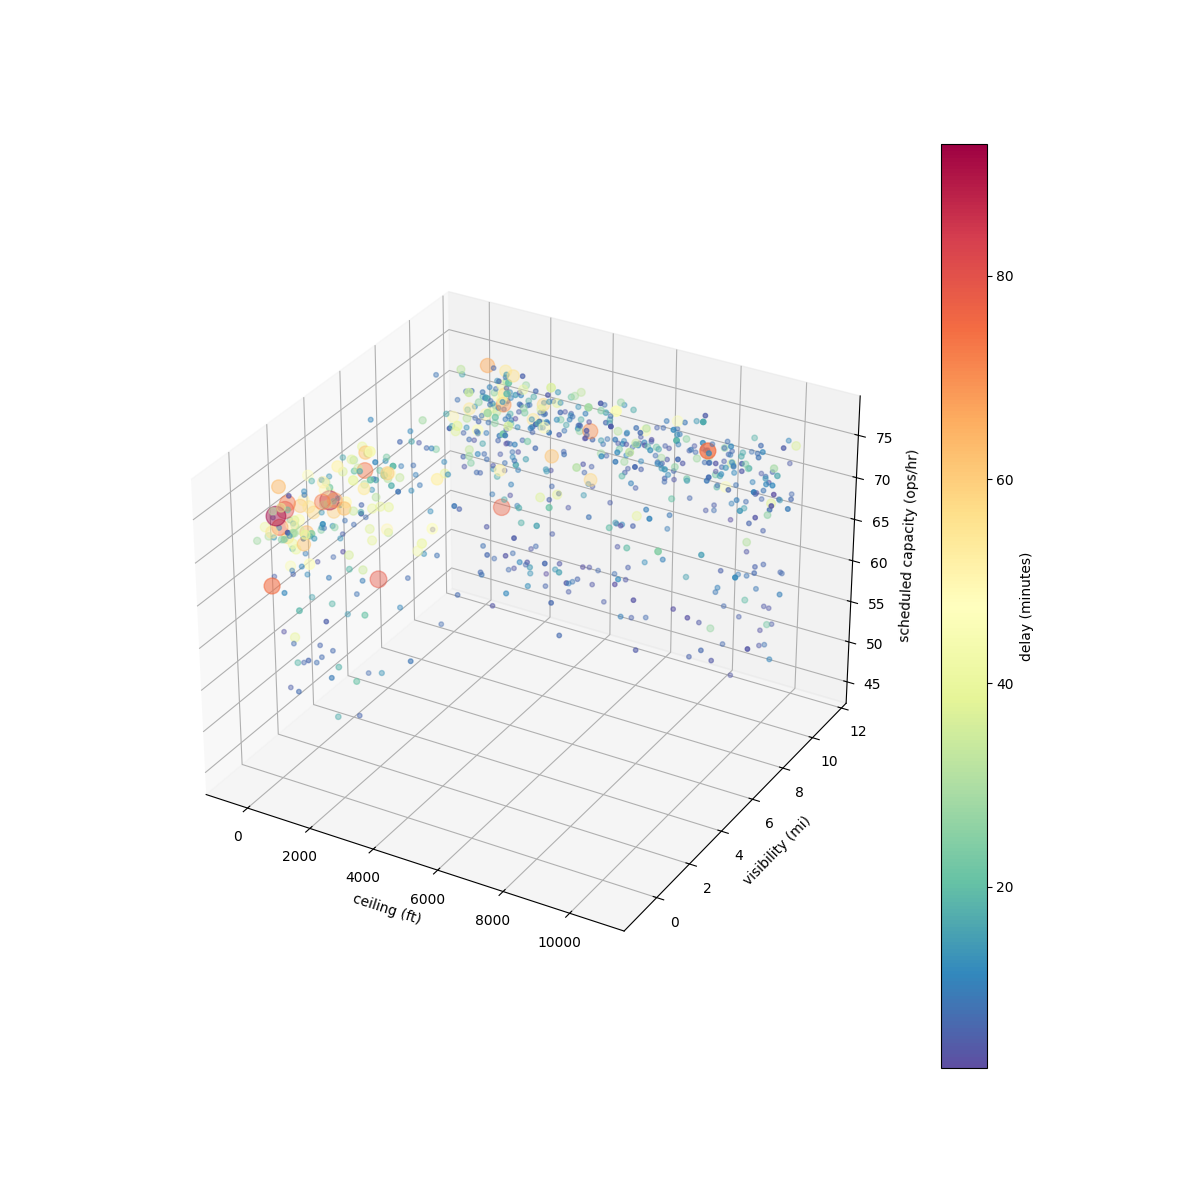
\includegraphics[width=\linewidth]{media/lga-analysis-17.png}
    \caption{3D scatter plot of both weather conditions and scheduled demand for each day in 2018 and 2019, where delay is represented with color. Points with higher delay also have greater size and opacity, for emphasis, and some noise is added for visualization purposes. }
    \label{fig:bubble3d-all}
\end{figure}

\begin{figure}[htb!]
    \centering
    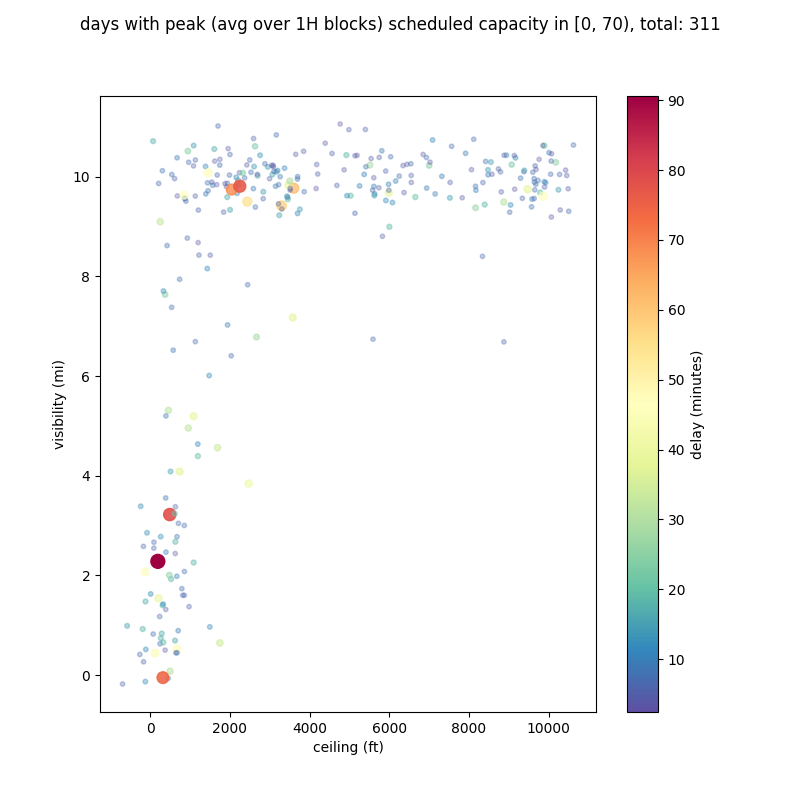
\includegraphics[height=8.0cm]{media/lga-analysis-15.png}
    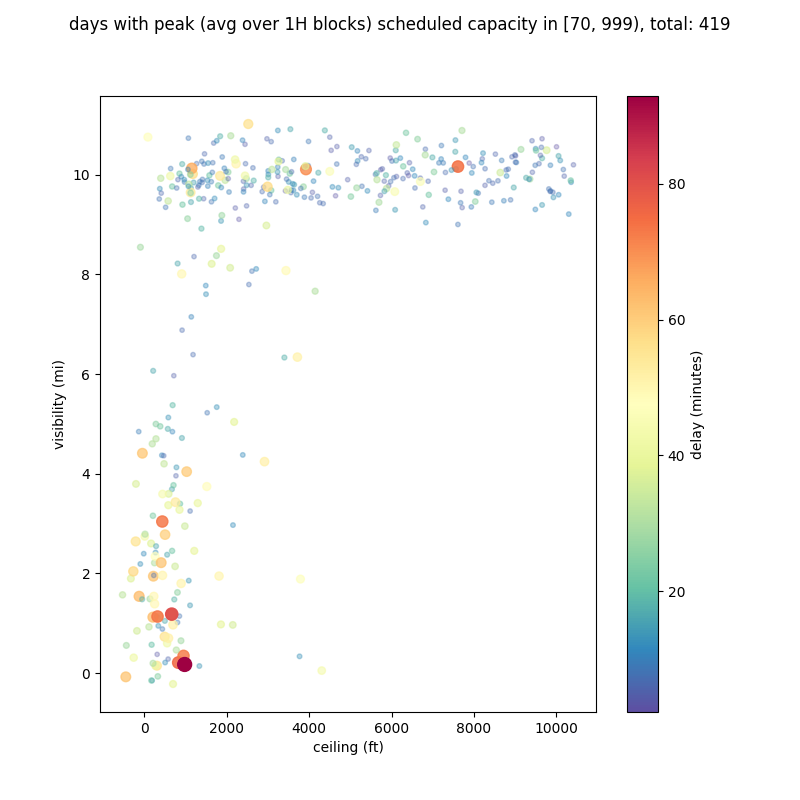
\includegraphics[height=8.0cm]{media/lga-analysis-16.png}
    \caption{Different distributions of delays given weather for lighter (left) and busier (right) days, which shows that failures are more concentrated in the region of higher demand and worse weather.}
    \label{fig:bubble2d-split}
\end{figure}

\subsection{Stochastic Airport Simulation}

We extend and adapt the stochastic queuing model developed in \cite{dawson2024breaking, michael_peng_probing_2024}, which was originally developed to study the mass cancellations and delays during the 2022 Southwest Airlines winter weather crisis, to better support our particular use case of less severe, but still impactful weather conditions. Specifically, we make two main changes.

The first is that we extend the model to be closer to reality, in terms of flights included. The original model only includes flights that have both endpoints, i.e. arrival and departure airport, within the set of 4 to 10 key network airports included. Additionally, only flights operated by Southwest are tracked. We add support for including all airline carriers present in the schedule data simultaneously, and also implement tracking for flights with one endpoint outside of the network. This is done by adding a source supernode, which emits all flights originating from outside the network to the relevant airports, and a sink supernode, to which all flights headed outside of the network are directed. The departure times at which flights are emitted from the source node are considered exogenous variables taken directly from the context, and we support a wide range of options including both scheduled and actual times. For this study, we choose to use the actual times, so that delays that are mainly attributable to LGA are properly modeled, and so that the demand profile of incoming flights when fitting our model is as realistic as possible.

The second change is that we add support for additional types of flight failures. The original simulation models delays and eager cancellations that result from when there are not enough available aircraft at an airport to depart at the scheduled time. We extend this to also model lazy cancellations, where flights that have been waiting to depart for long enough are canceled. Analogously, flights that have been waiting to arrive, which corresponds to waiting in holding patterns, are also considered failed after a given amount of time, because it is unrealistic for flights to wait for arrivals indefinitely. For this proof of concept, however, we disable both of these features, as minimal impact was observed in the very simplified scenario. Similarly, the actions taken, i.e. deciding which flights and when to cancel or delay, is set to the simple default strategy of first in first out (FIFO), but in future work, incorporating choice of strategy into the simulation will be important, as the end goal is stress-testing future design decisions.

With this in mind, our simulation roughly proceeds as follows. Flights are emitted from the source supernode at given times, to represent external incoming demand. The ego airport, which in this case is LGA, also has departing flights it must attempt to accommodate. When flights are ready to depart or arrive at the ego airport, they are entered into a service queue to await processing. We use a single M/M/1 queue for this, where a single server handles all flights regardless of their arrival or departure status. The time between arrivals and departures is drawn from an exponential distribution, where the mean $\lambda^{-1}$ is the latent mean service time parameter. This simulates a Poisson process with rate $\lambda$, which explains the connection between our introduced mean service time and the more commonly seen airport capacity or throughput. Roughly speaking, higher mean service times can lead to increased delays if severe enough, because it will mean that the airport may become unable to handle the demand of scheduled flights and must cancel or delay some in order to operate within its current limits. We also note that this service time is meant to encompass all factors that might affect throughput at a single airport, and not necessarily just the impact from visual versus instrument flight rules.

In this simplified setting, we directly bake in the notion of the action $\ra$ into the simulation, so we make no attempt to learn it implicitly. Similarly, we do not have any learned process parameters $\theta$ that are relevant to $\pld{x\given z;y}$, as we assume that we are working with a fully specified simulator. This is also implemented as a model through Pyro, a probabilistic programming language \cite{bingham2019pyro}, which makes the simulation differentiable, and gives us access to the likelihoods, so that we can use stochastic variational inference methods directly.

It is also important to reiterate here that mean service time on its own is not the only factor relevant to delays. \cref{fig:busy-light-comparison} shows two days that did not have significant delays in reality, after artificially imposing a higher mean service time of $0.2$ hours on both and simulating the result, and observing that the busier day was hit harder. This makes sense intuitively as well, because we would expect it to be easier to recover from a disruption with less external stress, so we can expect lighter days to be more tolerant to higher service times.

\begin{figure}[htb!]
    \centering
    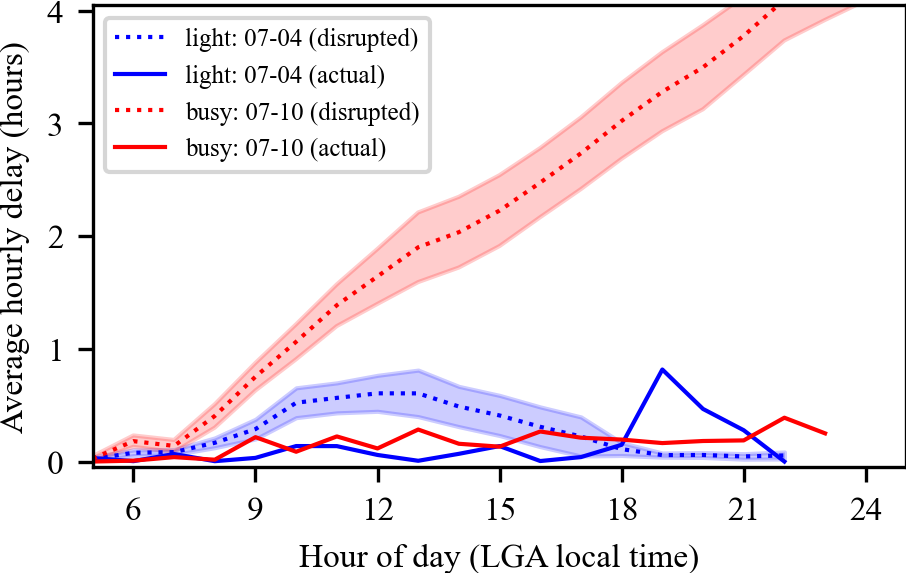
\includegraphics[width=0.7\linewidth]{media/busy_light_comparison.png}
    \caption{Demonstration of the effect of scheduled demand on delays on days with similar actual outcomes (solid lines). The same simulated disruption is applied to two days (dotted lines, shaded is standard deviation), showing that the lighter day (blue) is less affected than the busier (red).}
    \label{fig:busy-light-comparison}
\end{figure}

\subsection{Weather-Informed Priors}

We partially specify a simple mixture density model for the $\pld{z\given w}$ component. Specifically, we define a function $\fvn: w\mapsto c$ parameterized by $\nu$, where $c\in \ms C = \{0,1\}$ represents nominal and failure weather. 
\begin{proposition}[Weather Mixture Density Model]
    Then, we define our model as the following:
    \begin{equation}
        \pld{z\given w} = \begin{cases}
            \mt N(z;\mu_0, \sigma_0^2) \quad \text{if }\fvd{w} = 0\\
            \mt N(z;\mu_1, \sigma_1^2) \quad \text{if }\fvd{w} = 1,
        \end{cases}
    \end{equation}
    where $\mt N(\cdot;\mu,\sigma^2)$ denotes the univariate normal density with mean $\mu$ and variance $\sigma^2$.
\end{proposition}

We judgmentally select $\mu_0 = 0.012$ and $\sigma_0 = 0.001$ for nominal weather, and $\mu_1 = 0.019$ and $\sigma_1 = 0.001$ for failure weather, to incorporate the belief that worse weather leads to higher service times. 

\begin{proposition}[Relaxation of Threshold Classification for $\fvn$]
    For the decision function $\fvn$, we use a simple threshold classification given by
    \begin{align}
        \fvd{w} & = 1 - \sigma\left(\alpha (w_v-\wthvf)\right)\cdot \sigma\left(\alpha (w_c-\wthcf )\right) \\
        &\approx \begin{cases}
            1 \;\; \text{if} \;\; w_v \leq \wthvf \;\; \text{or}\;\;  w_c \leq \wthcf \\
            0 \;\; \text{otherwise}
        \end{cases}
    \end{align}
    where $\sigma(x)=(1+e^{x})^{-1}$ is the sigmoid function, and $\alpha = 50$ is a fixed scaling parameter to control the sharpness of the threshold.
\end{proposition}


Here, we let $w = (w_v, w_c) $, to represent the individual visibility and ceiling components, and let $\nu = (\wthvf,\wthcf)$ be thresholds parameterizing $\fvn$ that must be learned. We can interpret this model as imposing weather-informed priors on $z$ based on $w$, instead of just assuming the same prior for all observations, to incorporate the effect of weather. Additionally, we can extend this to the continuous case $\ms C=[0,1]$ directly by linearly interpolating between the nominal and failure density accordingly, as we will use in \cref{sec:atrds-theory}.

While we chose to specify all $\mu_c$ and $\sigma_c$, we also note that these can be set to different values, to investigate what the learned thresholds might be to decide between various severity levels of service time impact. 

\section{Toy Example -- Two Moons}
\label{sec:atrds-moons}
Before we move on, we present a simple toy example on the classic two moons dataset, which we augment with a weather-analogue variable. Here, we set $w\in [0,1]$, where being below a given threshold generates the nominal distribution of points in 2D space
\[
    \theta \sim \mt U(0, \pi),\quad \rx \sim\mt N(\cos\theta - 0.5, 0.1), \quad \ry \sim \mt N(\sin \theta - 0.25, 0.1)
\]
and being above the threshold generates the failure distribution from
\[
    \theta \sim \mt U(\pi, 2\pi),\quad \rx \sim\mt N(\cos\theta + 0.5, 0.1), \quad \ry \sim \mt N(\sin \theta + 0.75, 0.1),
\]
in the same way as \cite{dawson2025rare}, where $\mt U$ denotes the uniform distribution. We consider the actual point here to be the latent variable $z$, and add Gaussian noise to it to obtain observations $x$. Then, we attempt to learn an approximation for the posterior $\pld{z\given x,w}$, for each range of $w$, failure and nominal.

\begin{figure}[htb!]
    \centering
    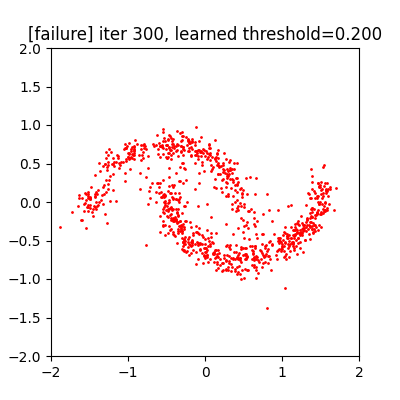
\includegraphics[height=7.5cm]{media/Figure_1A.300.png}
    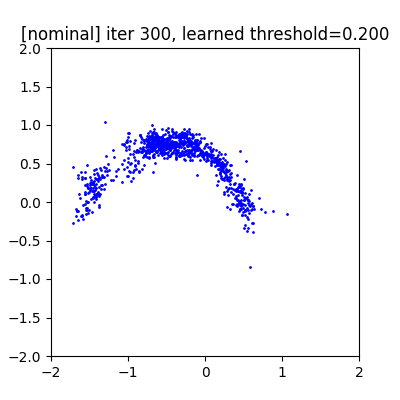
\includegraphics[height=7.5cm]{media/Figure_2A.300.png}
    \caption{Samples from two moons learned posteriors, with incorrectly specified threshold.}
    \label{fig:2moons-bad}
\end{figure}

\begin{figure}[htb!]
    \centering
    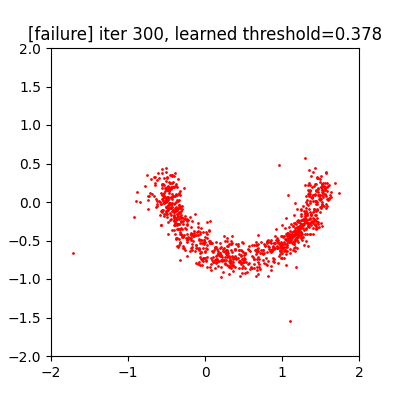
\includegraphics[height=7.5cm]{media/Figure_1.300.png}
    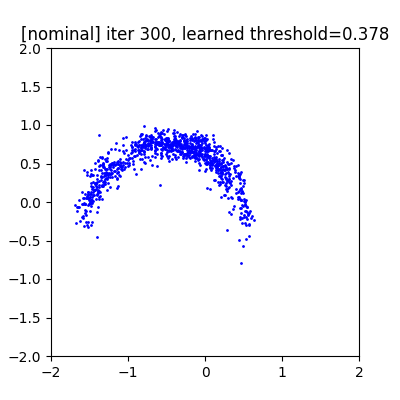
\includegraphics[height=7.5cm]{media/Figure_2.300.png}
    \caption{Samples from two moons learned posteriors, with correct learned threshold.}
    \label{fig:2moons-good}
\end{figure}

\cref{fig:2moons-bad} shows the result when the threshold is incorrectly specified, and \cref{fig:2moons-good} shows the result when the threshold is simultaneously learned. Here, we use a normalizing flows architecture to learn posteriors. As we can see, it is important to ensure that that if we are learning separate posteriors, that they are primarily learned on the data that we are interested in. In the case of the air traffic problem, it is part of the reason why it can be problematic to just classify days into failure or nominal purely based on observed delay or weather, because if our classification is wrong or we do not yet have a clear understanding of how those relate to different regions of the latent space, we may obtain inaccurate or less useful results.

\section{Theoretical Development}
\label{sec:atrds-theory}
\begin{figure} [htb!]
    \centering
    % feel free to improve this i don't actually know how to use this
    \tikz{
        % nodes
        \node[obs] (y) {$\rx$};%
        \node[latent,left=of y, xshift=-.4cm] (z) {$\rz$} ; %
        \node[obs,left=of z, xshift=-.4cm] (w) {$\rw$}; %

        % Factors
        \factor[left=of y, xshift=-.2cm] {z-y} {below:$\pld{x\given z;y}$} {} {} ; %
        \factor[left=of z, xshift=-.2cm] {w-z} {below:$\pld{z\given w}$} {} {} ; %

        \factor[above=of z, yshift=.1cm] {q} {above:$\qvd{z\given x,w;y} \approx \pld{z\given x,w;y}$} {} {} ; %
        \factor[below=of z, yshift=-.1cm] {r} {below:$\rvd{w\given x;y} \approx \pld{x\given w;y}$} {} {} ; %

        \node[const,above=of y, yshift=-.42cm] (y_above) {} ;
        \node[const,below=of y, yshift=.42cm] (y_below) {} ;
        \node[const,above=of w, yshift=-.42cm] (w_above) {} ;
        \node[const,below=of w, yshift=.42cm] (w_below) {} ;
        
        % % plate
        % \plate [inner sep=.25cm,yshift=.2cm] {plate1} {(x)(y)(z)} {$N$}; %
        % edges
        % \edge {w} {wt} ;
        % \edge {wt} {z} ;
        % \edge {z} {y} ;

        \edge[dashed, -] {w} {w_above} ;
        \edge[dashed, -] {y} {y_above} ;
        \edge[dashed] {w_below} {w} ;
        \edge[dashed, -] {y} {y_below} ;
        
        % factor edges
        % \factoredge[densely dashdotdotted] {w} {w-wt} {wt} ; %
        % \factoredge[densely dashdotdotted] {wt} {wt-z} {z} ; %
        \factoredge {w} {w-z} {z} ; %
        \factoredge {z} {z-y} {y} ; %

        \factoredge[dashed] {w_above,y_above} {q} {z} ; %
        \factoredge[dashed,-] {y_below} {r} {w_below} ; %
    }
    \caption{Overview of the probabilistic formulation for the proof of concept, with context $\ry$ omitted for clarity, showing where each of the variational approximations fit into the overall picture.}
    \label{fig:wzx-poc}
\end{figure}


As outlined in \cref{sec:intro-variants}, we will first need to learn posterior distributions $\pld{z\given x,w;y}$, while simultaneously fitting our model to historical observations. Then, we can use this learned model to predict effects of different conditions on a new day, or learn a different conditional density of interest. To this end, we apply stochastic variational inference, as introduced in \cref{background-variational-inference}, for the same reasons of computational tractability. In \cref{fig:wzx-poc}, we outline the distributions we are attempting to approximate. 

\subsection{Cluster Labels}

We will start with learning an approximation for latent posterior distribution $\qvd{z\given x,w;y}\approx \pld{z\given x,w;y}$. As discussed in \cref{sec:atrds-single-airport}, it is difficult to immediately identify which data points to group together for accurate learning of separate posteriors, so we will also learn a way to simultaneously cluster these points into groups, in a principled way, which also effectively also makes part of our learning problem unsupervised.

For this case study, we also adopt a simple threshold-based classification model. Specifically, we also select thresholds $\xth$ and $\yth$, and define a clustering function $\gvn:(x,y,w)\mapsto (d_x,d_y,d_w)=d$ as follows, with $x'$ and $y'$ as the result from aggregating $x$ and $y$ as described in \cref{sec:atrds-single-airport}:
\begin{proposition}[Partial Relaxation of Clustering for $\gvn$]
    We define our clustering function $\gvn$ as follows:
    \begin{align}
        \gvd{x,y,w}_x = d_x &= \mbm1_{x'\ge\xth}\\
        \gvd{x,y,w}_y = d_y &= \mbm1_{y'\ge\yth}\\
        \gvd{x,y,w}_w = d_w & = 1 - \sigma\left(\alpha (w_v-\wthvg)\right)\cdot \sigma\left(\alpha (w_c-\wthcg )\right) \\
        &\approx \begin{cases}
            1 \;\; \text{if} \;\; w_v \leq \wthvg \;\; \text{or}\;\;  w_c \leq \wthcg \\
            0 \;\; \text{otherwise.}
        \end{cases}
        % \begin{cases}
        %     1 \quad\text{if }\widetilde{x} \le\xth\\
        %     0 \quad{\text{otherwise}}
        % \end{cases}
    \end{align}
\end{proposition}

Here, $\mbm1$ is an indicator that takes on value $1$ when the condition is true and $0$ otherwise, and $\sigma(\cdot)$ is the sigmoid function.We use separate thresholds for the $w$ components in $\fvn$ and $\gvn$ because it is possible that the relevant thresholds for weather are different when also introducing contributions from other variables such as $y$. Similarly to $\fvn$, we set the parametrization for $\gvn$ as $\lambda = (\wthvg, \wthcg)$. In both $\fvn$ and $\gvn$, we use a smooth approximation for the weather threshold indicator to maintain differentiability, so the relevant ranges here are $c\in\ms C=[0,1]$ and $d\in \ms D=\{0,1\}\times \{0,1\}\times [0,1]$, where the $\times$ used here is the Cartesian product. 

By also learning this clustering, we can make sure that we are learning cleaner posteriors than if we had specified one beforehand that may or may not have been useful or just tried to learn on the entire dataset. It also allows us to perform amortized inference, because instead of just learning posteriors for our whole dataset $\Data$ or separate partitions of it, we instead learn separate posteriors conditioned on $d=\gvd{x,y,w}$ and the clustering function $\gvn$ at the same time, which means we can reuse our work and map new data points to a value of $d$ and use the relevant learned posterior, instead of having to do the learning process all over again.

It is also important to emphasize the difference between the cluster labels $d$ and the weather labels $c$, as they may appear to be the same at first glance. In particular, $c$ only depends on weather, and is only used in the forward direction of the $w\to z\to x$ model, so to speak. In contrast, $d$ depends on the entire data point $(x,y,w)$, and is used as a lower-dimensional label the learned posterior approximation $\qvn$ will be conditioned on.


\subsection{Variational Inference Setup}

Before we incorporate the labels $c$ and $d$, we will return to the general setting as shown in \cref{fig:wzx-poc} for a moment. Our problem differs somewhat from the standard variational inference setting, so we will provide derivations specific to our case for clarity. 

We assume $\rx,\rz,\rw$ are drawn from some true distribution $\ptd{\cdot;y}$, and we only have observations for $\rx$ and $\rw$. Then, as before, we let $\pld{\cdot;y}$ represent the learned model, in which we specify in two separate components for before and after the latent variable $\rz$.

In particular, $\pld{x\given z;y}$ may be specified by the simulated system dynamics, and $\pld{z\given w}$ by a specified model of the effect of weather conditions on the latent simulation parameters $z$. One benefit of this division is that dealing with the individual parts can be easier than trying to work with $w\to x$ directly, especially when the actual connection is not particularly clear, such as in our case.

Another benefit is that we immediately obtain a connection to the standard generative modeling setting by considering the relationship between individual parts of our model. Examining the joint distribution $\pld{x,z\given w;y}$, which may readily be rewritten as the product $\pld{x\given z;y}\pld{z\given w}$, a natural interpretation arises by considering the system dynamics of the simulation $\pld{x\given z}$ to be a standalone process, which uses weather-informed priors on the latent variables $\rz$ specified by $\pld{z\given w}$. However, it is important to note that while these specifications may be helpful in smoothly integrating domain knowledge into the model, it is not actually necessary to specify them, and our framework also encompasses a fully black-box treatment, as long as sufficient training data is available.

\begin{example}[Assortment of Conditional Densities]
    Here are some conditional densities obtained via Bayes' rule.
    \begin{align}
        \pld{x,w\given z;y} &= \pld{x\given z;y}\pld{w\given z}\\
        \pld{z,w\given x;y} &= \pld{w\given z}\pld{z\given x;y}\\
        \pld{x,z\given w;y} &= \pld{x\given z;y}\pld{z\given w}\\
        \pld{w\given x,z;y} &= \pld{w\given z} \\
        \pld{x\given z,w;y} &= \pld{x\given z;y} \\
        \pld{z\given x,w;y} &= \frac{\pld{x\given z;y}\pld{z\given w}}{\pld{x\given w}} = \frac{\pld{w\given z}\pld{z\given x;y}}{\pld{w\given x;y}}.
    \end{align}
\end{example}

Now, under this structure, there are a number of conditional distributions we may be interested in as an intermediate step, or even on their own, which we enumerate above.

Here, the two different forms for $\pld{z\given x,w;y}$, obtained through two equivalent applications of Bayes' rule, are particularly illuminating, as they reveal the connection between the individual edges of our probabilistic graphical model and the overarching goal of approximating $\pld{x\given w;y}$ and $\pld{w\given x;y}$. Specifically, suppose that we have learned a variational distribution that approximates $\qvd{z\given x,w;y}\approx \pld{z\given x,w;y}$, and let the optimal parametrization be
\[
    \hat\phi,\hat\theta = \argmin_{\phi,\theta} \DKL{\qvd{\cdot\given x,w;y}}{\pld{\cdot\given x,w;y}}.
\]
Then, we may use our two forms for $\pld{z\given x,w;y}$ to immediately obtain the following estimator
\begin{align}
    \log \pgdh{\hat\phi,\hat\theta}{x\given w;y} 
    &= \EX{\rz\sim\qgdh{\hat\phi}{\cdot\given x,w;y}}{\log\frac{\pgd{\hat\theta}{x,z\given w;y} }{\qgd{\hat\phi}{z\given x,w;y} } } \\
    &= \EX{\rz\sim\qgdh{\hat\phi}{\cdot\given x,w;y}}{\log\pgd{\hat\theta}{x\given w;y} + \log\frac{\pgd{\hat\theta}{z\given x,w;y} }{\qgd{\hat\phi}{z\given x,w;y} }} \\ 
    &= \log\pgd{\hat\theta}{x\given w;y} - \DKL{\qgd{\hat\phi}{\cdot\given x,w;y}}{\pgd{\hat\theta}{\cdot\given x,w;y}} \\ 
    &= \log\pgd{\hat\theta}{x\given w;y} - \min_{\phi,\theta} \DKL{\qgd{\phi}{\cdot\given x,w;y}}{\pgd{\theta}{\cdot\given x,w;y}}
\end{align}
and analagously,
\begin{align}
    \log \pgdh{\hat\phi,\hat\theta}{w\given x;y} 
    &= \EX{\rz\sim\qgdh{\hat\phi}{\cdot\given x,w;y}}{\log\frac{\pgd{\hat\theta}{z,w\given x;y} }{\qgd{\hat\phi}{z\given x,w;y} } } \\
    &= \EX{\rz\sim\qgdh{\hat\phi}{\cdot\given x,w;y}}{\log\pgd{\hat\theta}{w\given x;y} + \log\frac{\pgd{\hat\theta}{z\given x,w;y} }{\qgd{\hat\phi}{z\given x,w;y} }} \\ 
    &= \log\pgd{\hat\theta}{w\given x;y} - \DKL{\qgd{\hat\phi}{\cdot\given x,w;y}}{\pgd{\hat\theta}{\cdot\given x,w;y}} \\ 
    &= \log\pgd{\hat\theta}{w\given x;y} - \min_{\phi,\theta} \DKL{\qgd{\phi}{\cdot\given x,w;y}}{\pgd{\theta}{\cdot\given x,w;y}}.
\end{align}

Hence, finding $\phi,\theta$ such that $\qvd{z\given x,w;y}$ is a close approximation for the posterior distribution $\pld{z\given x,w;y}$, in terms of minimizing the KL-divergence between $\qvd{\cdot}$ and $\pld{\cdot}$, will also immediately yield estimators $ \pgdh{\hat\phi,\hat\theta}{x\given w;y} $ and $ \pgdh{\hat\phi,\hat\theta}{w\given x;y} $. Although these estimators are biased downward except in the case of $\qvd{z\given x,w;y}=\pld{z\given x,w;y}$, the derivation above shows that they at least achieve minimal bias among all estimators of their particular family parametrized on $\phi,\theta$, and are easy to compute, provided that sampling from $\qvd{\cdot}$ is easy, which is a criteria for a good variational family anyway.

\begin{proposition}[Biased Density Estimators]
    Putting our results from above together, we have
    \begin{align}
    \log \pgdh{\hat\phi,\hat\theta}{x\given w;y}    
    &= \log\pgd{\hat\theta}{x\given w;y} - \min_{\phi,\theta} \DKL{\qgd{\phi}{\cdot\given x,w;y}}{\pgd{\theta}{\cdot\given x,w;y}}\\
    \log \pgdh{\hat\phi,\hat\theta}{w\given x;y} 
    &= \log\pgd{\hat\theta}{w\given x;y} - \min_{\phi,\theta} \DKL{\qgd{\phi}{\cdot\given x,w;y}}{\pgd{\theta}{\cdot\given x,w;y}}. 
\end{align}
\end{proposition}

One caveat is that we don't have both estimators completely for free. While our estimator for the predictive distribution $\pgdh{\hat\phi,\hat\theta}{x\given w;y}$ only requires $\pld{x,z\given w;y}=\pld{x\given z;y}\pld{z\given w}$, where both individual predictive components are assumed to be tractable, the estimator for the posterior $\pgdh{\hat\phi,\hat\theta}{w\given x;y}$ requires $\pld{z,w\given x;y}=\pld{w\given z}\pld{z\given x;y}$, where both individual posterior components are intractable in general. There are a few different ways around this. The first is to restrict our model to so that each individual prior and posterior pair are conjugate distributions, so that the posterior is analytically tractable as well.

Alternatively, if we do not wish to impose such a strong limitation, we may instead learn a variational approximation for either the posteriors $\pld{w\given z}$ and $\pld{z\given x;y}$ individually, or the single joint posterior $\pld{z,w\given x;y}$. Similarly, we can also leverage our approximation for $\pld{x\given w;y}$ to directly learn a variational approximation for $\pld{w\given x;y}$. Finally, in some special cases, it is not necessarily that difficult to directly compute the individual posteriors $\pld{w\given z}$ and $\pld{z\given x;y}$, even if the result of marginalizing their product over $\rz$ may not be tractable.

To summarize, here are the main steps of learning conditional distributions of weather given observed delays, or vice versa, assuming that we have access to some partially specified individual components:

\begin{enumerate}
    \item Provide a parametrization by $\theta$ for $\pld{y\given z}$ and $\pld{z\given w}$, though the optimal values for $\theta$ do not need to be known, which we have already done for our problem in \cref{sec:atrds-single-airport}
    \item Learn a variational approximation $\qvd{z\given x,w;y}\approx\pld{z\given x,w;y}$, as in \cref{background-variational-inference}.
    \item Using $\qvd{\cdot}$, obtain variational approximations for distributions $\pld{x\given w;y}$ and $\pld{w\given x;y}$.
\end{enumerate}


\subsection{Variational Inference Details}

For the second step, we construct the evidence lower bound objective in the standard manner, which is presented here for clarity. 

\begin{proposition}[Maximum Likelihood Objective]
    Starting with the maximum likelihood objective, we wish to find $\theta$ that maximizes
    \[
        \EX{\rx,\rw\sim\ptd{\cdot, \cdot;y}}{\log \pld{x,w;y}} = -H(\ptd{\cdot,\cdot;y})-\DKL{\ptd{\cdot,\cdot;y}}{\pld{\cdot,\cdot;y}}.
    \]
\end{proposition}

Here, we note the well-known result that maximizing the log-likelihood is equivalent to minimizing the KL-divergence between the learned and true data distribution. Because the true data distribution $\ptd{\cdot}$ is unknown, we use the approximation given by the empirical distribution $\ped{\cdot;\Data}$ of our dataset $\Data$ instead. Now, let us consider the term inside the expectation $\log \pld{x,w;y}$, which, after artificially taking the expectation over $\rz$, can be decomposed into
\begin{align*}
    % &\phantomeq\log \pld{y,w} \\
    % &= 
    &\phantomeq\EX{\rz \sim \qvd{\cdot\given x,w;y} }{\log\pld{x,w;y} } \\
    &= \EX{\rz \sim \qvd{\cdot\given x,w;y} }{\log\frac{\pld{x,w;y}\qvd{z\given x,w;y}}{\pld{x,z, w;y}}\cdot\frac{\pld{x,z,w;y}}{\qvd{z\given x,w;y}} } \\
    &= \EX{\rz \sim \qvd{\cdot\given x,w;y} }{\log\frac{\qvd{z\given x,w;y}}{\pld{z\given x,w;y}}+\log\frac{\pld{x,z,w;y}}{\qvd{z\given x,w;y}}} \\
    &= \underbrace{\DKL{\qvd{\cdot\given x,w;y}}{\pld{\cdot\given x, w;y}}}_{\text{KL-divergence term}} + \underbrace{\EX{\rz \sim \qvd{\cdot\given x,w;y} }{ \log\frac{\pld{x,z,w;y}}{\qvd{z\given x,w;y}}}}_{\text{ELBO term: }\elbo{q}{\phi, \theta, x, w;y}}
\end{align*}

Our focus is on the ELBO term $\elbo{q}{\phi, \theta, x, w;y}$, which serves as a lower bound for the log-likelihood $\log\pld{x,w;y}$. Because maximizing the ELBO is equivalent to simultaneously minimizing the KL-divergence term and maximizing the log-likelihood objective, our goal is to solve the optimization problem
\begin{align*}
    \hat\phi,\hat\theta &= \argmax_{\phi,\theta} \EX{\rx,\rw,\ry \sim\ped{\cdot, \cdot, \cdot; \Data}}{\elbo{q}{\phi,\theta, x,w;y}} \\
    &= \argmax_{\phi,\theta} \frac1{|\Data|} \sum_{(x,y,w)\in \Data} \elbo{q}{\phi,\theta,x,w;y}.
\end{align*}


\subsection{Incorporating Weather Labels}

Here is where our derivation differs further from the standard case. First, we interpret the mapping $\fvn :w\mapsto c$, as assigning a regime, or mixture of regimes, to each data point, which governs the learned distributions it is supposed to follow, through the weather-based prior interpretation. In particular, we may rewrite our per-observation ELBO as:
\begin{equation}
    \elbo{q}{\phi, \theta, x; c, y} = \EX{\rz \sim \qvd{\cdot\given x;c,y} }{ \log\frac{\pld{x,z;c,y} }{\qvd{z\given x; c,y}}},
\end{equation}
and rewrite the corresponding optimization problem as 
\begin{equation}
    \hat\phi,\hat\theta,\hat\nu = \argmax_{\phi,\theta,\nu} \sum_{(x,y,w)\in \Data} \elbo{q}{\phi,\theta,x;\fvd{w},y},
\end{equation}
where we drop the constant multiplicative term because it does not affect the result. 

\begin{proposition}[ELBO with Weather Labels]
    In fact, we can also write
    \begin{align*}
        \elbo{q}{\phi, \theta, x; c,y} &= \EX{\rz \sim \qvd{\cdot\given x;c,y} }{ \log\frac{\pld{x\given z,y}\pld{z;c} }{\qvd{z\given x; c,y}}} \\
        &= \underbrace{\EX{\qvd{\cdot\given x;c,y} }{ \log\pld{x\given z;y} }}_{\text{maximum likelihood term}} - \underbrace{\DKL{\qvd{\cdot\given x;c,y}}{\pld{\cdot;c,y}}}_{\text{KL-divergence term}}
    \end{align*}
\end{proposition}

This shows that maximizing $\elbo{q}{\phi,\theta,y,c}$ is equivalent to maximizing the likelihood of the posterior predictive distribution, with an additional prior regularization term that penalizes the variational distribution from diverging farther from the weather-informed prior. 

Now we consider the third step of our method, which is leveraging our results from the previous step to approximate $\pld{w\given x;y}$. In our particular case, we may apply the following:
\begin{align}
    \pld{w\given x;y} &= \sum_{c\in\ms C} \pld{w\given c}\pld{c\given x;y}\\
    &= \sum_{c\in\ms C} \pld{w\given c}\cdot\frac{\pld{x;c,y}\pld{c}}{\sum_{c\in\ms C} \pld{x;c,y}} \\
    &= \frac{\pld{x;\fvd{w},y}\pd{w}}{\sum_{c\in\ms C} \pld{x;c,y}}
\end{align}
where $\pld{c\given w}=\pld{w\given c}=\mathbbm{1}_{c=\fvd{w}}$, because $\fvn$ is deterministic by definition. The normalization term in the denominator is a tractable sum as long as $|\ms C|$ is not very large, and we can also estimate $\pld{x;c,y}$ using $\qvd{z\given x;c,y}$ as we showed before.

However, in terms of interpretable results, this exact distribution is perhaps not the most useful for our analysis. Instead, it is more natural to consider the learned posteriors $\qvd{z\given x;c,y}$, under the failure and nominal weather regimes which induce their respective weather-informed priors $\qvd{z\given c}$, along with the learned $\fvn$, which determines regions over the $\rw$ space that map to the aforementioned failure and nominal weather regimes. This can interpreted as assuming that we have a different failure and nominal distributions, and aiming to simultaneously learn how to classify a new observation as failure and nominal, and the corresponding approximate posteriors for the failure and nominal observations.

\subsection{Incorporating Cluster Labels}

We can similarly incorporate our cluster label determined by $\gvn$, and re-write our per-observation ELBO one more time as 
\begin{equation}
    \elbo{q}{\phi, \theta, x; c,d,y} = \EX{\rz \sim \qvd{\cdot ;c,d} }{ \log\frac{\pld{x\given z;y}\pld{z; c} }{\qvd{z; d}}}.
\end{equation}

\begin{proposition}[Overall Optimization with Weather and Cluster Labels]
    Then, the corresponding overall optimization problem as 
    \begin{equation}
        \hat\phi,\hat\theta,\hat\nu,\hat\gamma = \argmax_{\phi,\theta,\nu,\gamma} \sum_{(x,y,w)\in \Data} \elbo{q}{\phi,\theta,x;\fvd{w},\gvd{x,y,w}, y}.
    \end{equation}
\end{proposition}

\subsection{Performance Engineering}

We can make some additional optimizations to reduce training time, by noticing that the main potential bottleneck in our ELBO for individual observations is the $\pld{x,z;c,y}$ term in the numerator, because depending on the implementation and fidelity of the simulation, evaluating likelihoods from a simulation trace and computing all of the gradients may be computationally expensive. To avoid having to re-do this for every subsample at each training step, we write
\begin{equation}
    \pld{x\given z;y}\pld{z;c} = \pld{x,z;c,y} = \pld{z\given x;c,y}\pld{x;c,y}.
\end{equation}
Therefore, we may rewrite our per-subsample ELBO as
\begin{align}
    \elbo{q}{\phi, \theta, x ; c,d,y} &= \EX{\rz \sim \qvd{\cdot ;d} }{ \log\frac{\pld{z\given x;c,y}\pld{x;c,y} }{\qvd{z; d}}} \\
    &=\EX{\rz \sim \qvd{\cdot ; d} }{ \log\frac{\pld{z\given x;c,y} }{\qvd{z; d}}} +\log \pld{x;c,y}\\
    &= \log \pld{x;c,y} - \DKL{\qvd{\cdot ; d}}{\pld{\cdot \given x;c,y}}
\end{align}
One benefit is that we may now pre-compute $\log \pld{x;c,y}$ as
\begin{equation}
    \log \pld{x;c,y} = \EX{\rz \sim \pld{z;c}}{\log \pld{x\given z;y}},
\end{equation}
because the weather-informed priors $\pld{z;c}$ are specified beforehand, and $\pld{x\given z,y}$ depends only on the simulation. Hence, we only need to compute or estimate this once for each $c\in\ms C$ and each value of $y$ that appears in $\Data$ at the start, and then reuse these likelihoods throughout training. Because we allow $c$ to be continuous, we will instead compute this for only $c=\{0,1\}$, and interpret $c\in(0,1)$ as a linear mixture of those two distributions.

Furthermore, we can also learn a variational approximation $\svd{z\given x;c,y}$ for smaller subsamples of the full dataset, which in our case we will choose to be a single day, and use these to approximate $\pld{z\given x;c,y}$. This can be seem as intentionally over-fitting many separate learned posteriors to our individual subsamples, and then leveraging these in our combined objective to simultaneously learn accurate posteriors for labels $d$ that encompass than one sub-sample, while simultaneously learning $\gvn$ to best reflect whatever structure may exist in the data. Because all of these individual $\svn$ are completely independent of each other, we can learn them all in parallel, which allows us to more easily scale up to larger datasets. An example of some individual posteriors $\svn$ is shown in \cref{fig:s-phi-selection} and \cref{tab:s-phi-selection}

\begin{figure}
    \centering
    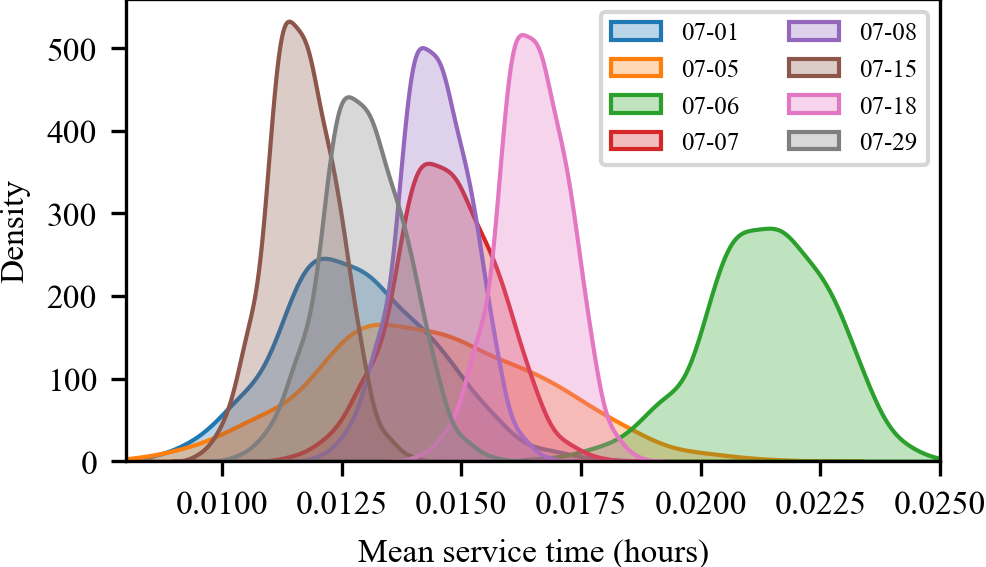
\includegraphics[width=0.8\linewidth]{media/s_phi_2019-07_selection.png}
    \caption{A selection of separate posterior approximations for individual subsamples of the full dataset, each corresponding to a single day from July 2019, as listed in the legend.}
    \label{fig:s-phi-selection}
\end{figure}


\begin{table}[htb]
    \centering
    \begin{tabular}{|c||c|c|}
        \hline
        Date & $\hat\mu$ (hrs) & $\hat\sigma$ (hrs) \\
        \hline\hline 
        2019-07-01 & 0.01283 & 0.002107 \\
        \hline
        2019-07-05 & 0.01427 & 0.002271 \\
        \hline 
        2019-07-06 & 0.02123 & 0.002229 \\
        \hline
        2019-07-07 & 0.01472 & 0.002315 \\
        \hline
        2019-07-08 & 0.01451 & 0.002305 \\
        \hline 
        2019-07-15 & 0.01181 & 0.001953 \\
        \hline
        2019-07-18 & 0.01650 & 0.002414 \\
        \hline
        2019-07-29 & 0.01305 & 0.002140 \\
        \hline
    \end{tabular}
    \caption{Estimated mean $\hat\mu$ and standard deviation $\hat\sigma$ in hours for daily posteriors $\svn$.}
    \label{tab:s-phi-selection}
\end{table}


\subsection{Final Loss Construction}

This breaks up our optimization problem into two steps. First, we wish to find individual
\begin{equation}
    \hat\psi^{(k)}, \hat\theta^{(k)} = \argmax_{\psi,\theta} \underbrace{\EX{\rz\sim\svd{\cdot\given x^{(k)};c^{(k)}, y^{(k)}}}{\log\frac{\pld{x^{(k)}\given z, y^{(k)}}\pld{z;c^{(k)}}}{\svd{z\given x^{(k)};c^{(k)}, y^{(k)}}}}  }_{\elbo{s}{\psi, \theta, x^{(k)}; c^{(k)}, y^{(k)}}}
\end{equation}
for each $(x^{(k)},w^{(k)}, y^{(k)})\in\Data$, where $c^{(k)}=\fvd{w^{(k)}}$. For clarity, we re-iterate that we have specifically learned these variational approximations $\svd{z\given y;c}$ for each $y$ and $c$, and $\svn$ does not immediately accept $y$ as an input. Also, in our case, $\theta$ as pertains to $\pld{x\given z;y}$ is assumed to be empty, so we are really just finding $\hat\psi^{(k)}$. Once we have learned these, we then approximate
\begin{equation}
    \elbo{q}{\phi,\theta,x;c,d,y}\approx \log \pld{x;c,y} - \DKL{\qvd{\cdot ; d}}{\svd{\cdot \given x;c,y}},
\end{equation}

and just use this as usual in our previously derived
\begin{equation}
    \hat\phi,\hat\theta,\hat\nu,\hat\gamma = \argmax_{\phi,\theta,\nu,\gamma} \sum_{(x,y,w)\in \Data} \elbo{q}{\phi,\theta,x;\fvd{w},\gvd{x,y,w},y}.
\end{equation}

\begin{proposition}[Final Loss Construction]
    To fit loss conventions, we negate this and instead solve the mirrored problem
    \begin{equation}
        \hat\phi,\hat\theta,\hat\nu,\hat\gamma = \argmin_{\phi,\theta,\nu,\gamma} \sum_{(x,y,w)\in \Data} -\elbo{q}{\phi,\theta,x;\fvd{w},\gvd{x,y,w},y}.
    \end{equation}    
\end{proposition}



\section{Implementation Details}
\label{sec:atrds-implementation}
For learning the individual posteriors $\svd{z\given x;c,y}$ for each $(x,y,w)\in\Data$ and $c\in \{0,1\}$, we use Pyro's SVI library \cite{bingham2019pyro}, to smoothly integrate with our air traffic simulation which is implemented as a probabilistic model in the same language. We use a multivariate Gaussian distribution as the variational family, automatically transformed to fit a positivity constraint we place on the mean service time $z$ in the probabilistic program.

For learning $\qvd{z;c,d}$, we use a conditional normalizing flow as the variational family. Specifically, we use the neural spline flow architecture \cite{durkan2019neural} with $3$ stacked transforms, and $2$ hidden layers of $16$ units each, using a Rectified Linear Unit (ReLU) activation. The context dimension for conditioning is $5$, where the first four entries represent a one-hot encoding for $d$ through each combination of the $d_x$ and $d_y$ components, and the fifth entry is the $d_w$ component, given by $\gvn$. In other words, we transform the 3-dimensional label $d$ to a 5-dimensional label $\widetilde{d}$, only for training the normalizing flow to encourage further decoupling of the clusters, as show in \cref{tab:d-training-labels}.
% \begin{align}
%     d = (0,0,d_w)&\implies (1,0,0,0,d_w)=\widetilde{d},\\
%     d = (0,1,d_w)&\implies (0,1,0,0,d_w)=\widetilde{d},\\
%     d = (1,0,d_w)&\implies (0,0,1,0,d_w)=\widetilde{d},\\
%     d = (1,1,d_w)&\implies (0,0,0,1,d_w)=\widetilde{d}.
% \end{align}

\begin{table}[htb]
    \centering
    \begin{tabular}{c||c}
        $d$ & $\widetilde{d}$ \\
        \hline\hline
        $(0,0,d_w)$ & $(1,0,0,0,d_w)$ \\
        \hline
        $(0,1,d_w)$ & $(0,1,0,0,d_w)$ \\
        \hline
        $(1,0,d_w)$ & $(0,0,1,0,d_w)$ \\
        \hline
        $(1,1,d_w)$ & $(0,0,0,1,d_w)$ \\
    \end{tabular}
    \caption{Corresponding training label $\widetilde{d}$ for each cluster label $d$.}
    \label{tab:d-training-labels}
\end{table}

We directly implement everything for this part in PyTorch, using the Zuko library for the normalizing flows architecture \cite{rozet2024probabilists}.

For optimization, we use the Adam optimizer with an initial learning rate $5\times 10^{-3}$ and an exponential decay schedule with final learning rate $10^{-3}$. For all SVI parameters, we clip gradient norms at $100$, and all classification parameters at $10$. The $\svn$ training process is run for $500$ iterations, and the $\qvn$ training process is run for $1000$ iterations, where $\phi$ is frozen at step $500$ to allow some time for $\nu$ and $\gamma$ to fully stabilize.

\section{Results and Discussion}
\label{sec:atrds-results}
After learning our separate posteriors and clustering $\gvn$, along with the weather thresholds used in $\fvn$, we can now analyze and apply our results to our original goals of understanding and generating failure conditions.

\subsection{Analyzing Learned Posteriors}

For our two user-defined parameters, we choose $\xth=15$ minutes for our delay threshold and $\yth=72$ operations per hour for our demand threshold in $\gvn$. For both $\fvn$ and $\gvn$, we use $\alpha=50$ as the boundary sharpness scaling parameter. Although LGA is currently supposed to have hourly limits of 71 for scheduled operations and 3 for unscheduled operations during slot-controlled hours, historical practices still allow for scheduled operations to be between 72 and 75 in most hours \cite{faa_lga_2024}. The final results of the learned parameters are
% \begin{align}
%     \wthvf&=1.392,\qquad
%     \wthcf=1318,\qquad\\
%     \wthvg&=1.600,\qquad
%     \wthcg=1276,
% \end{align}
\begin{table}[htb!]
    \centering
    \begin{tabular}{|c||c|c||c|c|}
        \hline
        Parameter & Value & Units & Type & Function\\
        \hline\hline
        $\wthvf$ & $1.392$ & miles & visibility & $\fvn$ \\
        \hline
        $\wthvg$ & $1.600$ & miles & visibility & $\gvn$ \\
        \hline\hline
        $\wthcf$ & $1318$ & feet & ceiling & $\fvn$ \\
        \hline
        $\wthcg$ & $1276$ & feet & ceiling & $\gvn$ \\
        \hline
    \end{tabular}
    \caption{Final learned visibility and ceiling thresholds}
    \label{tab:learned-thresholds}
\end{table}

where $\wthvf$ and $\wthvg$ are in statute miles and $\wthcf$ and $\wthcg$ are in feet. Our final ELBO loss, i.e. negated ELBO, was $-204.34$ nats/dim. \cref{fig:q-phi-combined} shows the posterior distributions for the learned mean service times constructed from $10000$ samples for each cluster determined by $d= \gvd{x,y,w}$, for each of the eight labels $d\in \{0,1\}^3$, and \cref{tab:q-phi-results} displays some summary statistics. We can see that the posteriors appear to be reasonable, because the more nominal posteriors are near $0.0125$ hours, a mean service time which corresponds to a realistic capacity of $80$ operations per hour for LGA.

\begin{figure}[htb!]
    \centering
    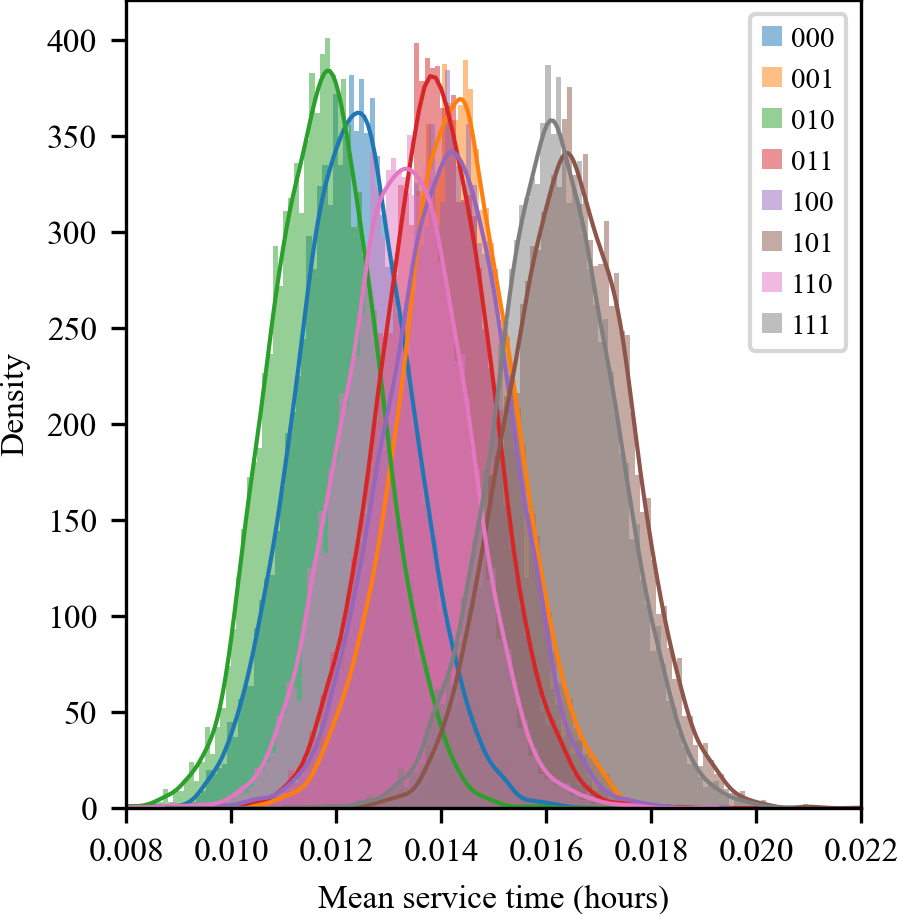
\includegraphics[height=3.0in]{media/q_phi_nsf_730_all.png}
    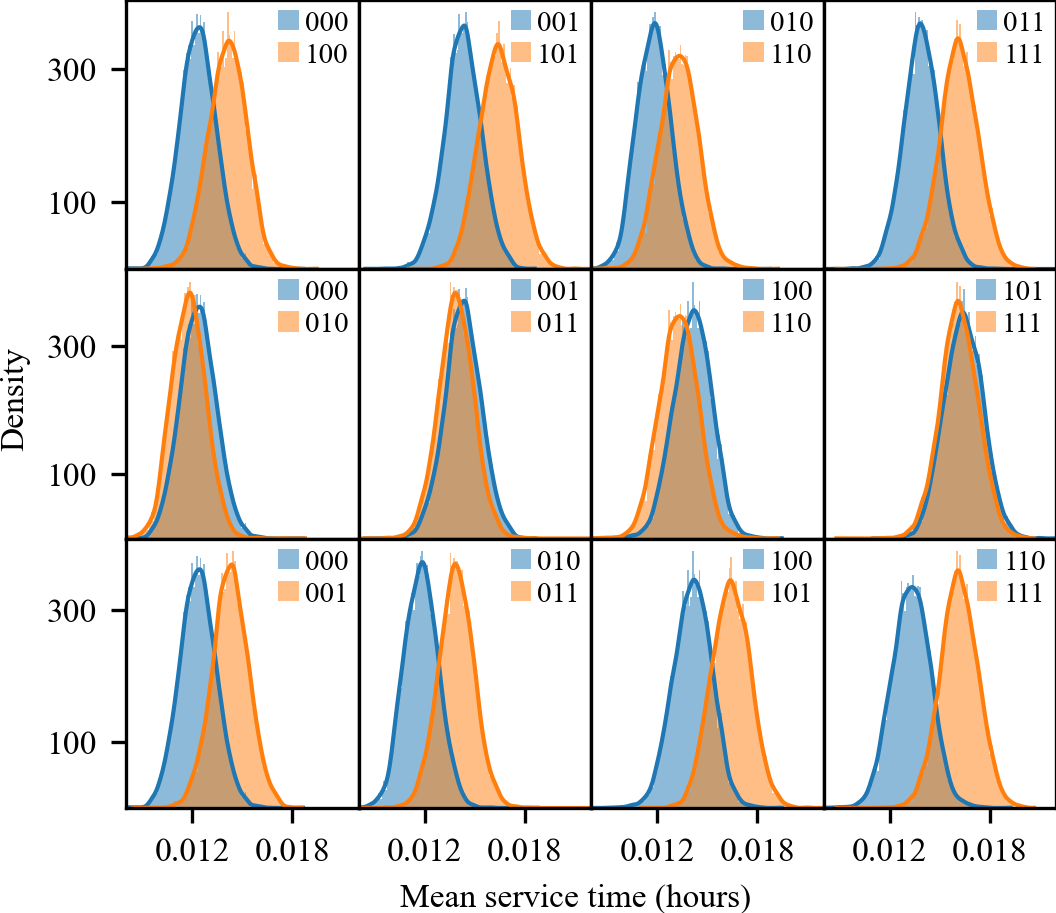
\includegraphics[height=3.0in]{media/q_phi_nsf_730_grid.png}
    \caption{Variational approximations for the mean service time $\rz$, for eight cluster labels $d\in\{0,1\}^3$. On the left, we plot the posteriors for all eight clusters for comparison. On the right, we plot pairs where two components of the label are held constant for each value in $\{0,1\}^2$ across the row, and the third is varied between $\{0,1\}$, with $d_x$, $d_y$, and $d_w$ being varied in the first, second, and third rows, respectively.}
    \label{fig:q-phi-combined}
\end{figure}

% 000 posterior, mean=0.01234, std=0.00110
% 001 posterior, mean=0.01429, std=0.00111
% 010 posterior, mean=0.01178, std=0.00104
% 011 posterior, mean=0.01389, std=0.00109
% 100 posterior, mean=0.01411, std=0.00116
% 101 posterior, mean=0.01643, std=0.00116
% 110 posterior, mean=0.01329, std=0.00117
% 111 posterior, mean=0.01617, std=0.00115

\begin{table}[htb]
    \centering
    \begin{tabular}{|c|c|c||c|c|}
        \hline
        $d_x$ & $d_y$ & $d_w$ & $\hat\mu$ (hrs) & $\hat\sigma$ (hrs) \\
        \hline\hline
        0 & 0 & 0 & 0.01234 & 0.00110 \\
        \hline
        0 & 0 & 1 & 0.01429 & 0.00111 \\
        \hline
        0 & 1 & 0 & 0.01178 & 0.00104 \\
        \hline
        0 & 1 & 1 & 0.01389 & 0.00109 \\
        \hline
        1 & 0 & 0 & 0.01411 & 0.00116 \\
        \hline
        1 & 0 & 1 & 0.01643 & 0.00116 \\
        \hline
        1 & 1 & 0 & 0.01329 & 0.00117 \\
        \hline
        1 & 1 & 1 & 0.01617 & 0.00115 \\
        \hline
    \end{tabular}
    \caption{Estimated mean $\hat\mu$ and standard deviation $\hat\sigma$ in hours for learned posteriors $\qvn$.}
    \label{tab:q-phi-results}
\end{table}

Using the pairwise comparison plots in the grid on the right side of \cref{fig:q-phi-combined}, we can investigate the effect of each component of $d$ on the learned posterior for its cluster. In the first row, where only $d_x$ is varied in each plot, we note that the posteriors for $d_x=0$ (blue) are to the left of those for $d_x=1$ (orange). This shows that introducing more delays corresponds to shifting the learned posterior to the right, which is what we expected to see. Similarly, in the third row, where only $d_w$ is varied in each plot, we note that the posteriors for $d_w=0$ (blue) are to the left of those for $d_w=1$ (orange), which also aligns with the belief that worse weather leads to higher service times that we incorporated into the model.

In the second row, where only $d_y$ is varied in each plot, we observe a slightly different effect, although it is a bit less evident. Here, the posteriors for $d_y=0$ (blue) appear to be shifted to the right, in comparison to $d_y=1$ (orange). However, this still makes sense, because it is showing the effect of scheduled demand on delay that we had previously discovered in \cref{sec:atrds-single-airport}, that because of the higher scheduled demand, a lower mean service time may be required to achieve the same performance in terms of delays on a busier day versus a lighter one, all else held equal, which manifests here as the posterior for that particular cluster being shifted to the left slightly.


\subsection{Using Learned Posteriors}

Now that we have learned posteriors for our separate clusters, we can use them in our learned generative model, and analyze the results, similar to sampling from the posterior predictive distribution after learning an approximation for the posterior. 

\begin{figure}[htb!]
    \centering
    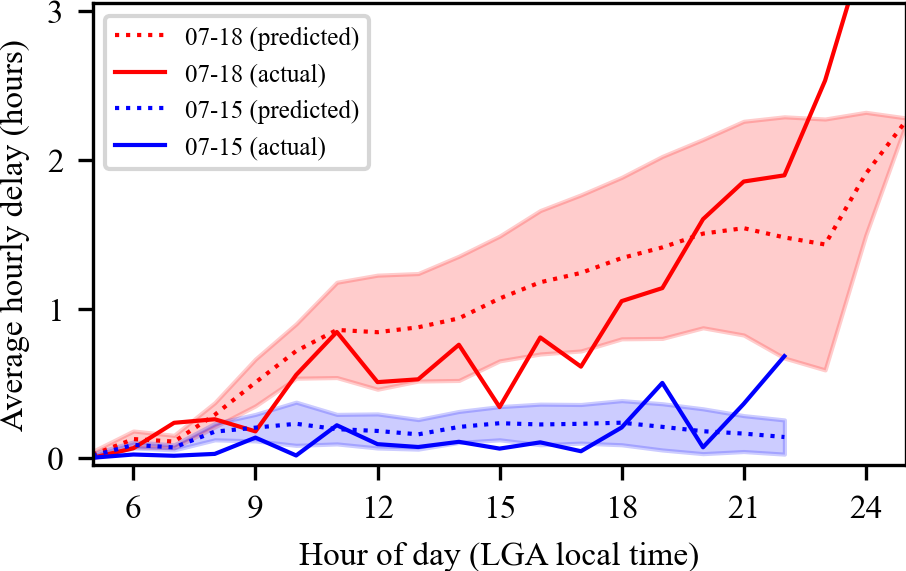
\includegraphics[width=0.7\linewidth]{media/posterior_predictive_comparison.png}
    \caption{Actual and predicted mean hourly delays using our model, with a weather-induced delay applied on one day (red) and nominal operations on the other (blue).}
    \label{fig:pp-comparison}
\end{figure}

We first select two days for analysis, which are July 18, 2019 (day 1) and July 15, 2019 (day 2). For both days, the peak scheduled hourly demand is $75$ operations, which is above $\yth$, so $d_{y,1}=d_{y,2}=1$. Additionally, the weather values for each day are $w_1=(10.0, 8649.3)$ and $w_2=(2.414,299.2)$, so $d_{w,1}\approx 0$ and $d_{w,2}\approx 1$. In reality, day 1 (red) has high delays above $\xth$, while day 2 (blue) does not, as seen in the solid lines in \cref{fig:pp-comparison}, so for comparison, we also select $d_{x,1}=1$ and $d_{x,2}=0$. Then, using each of these posteriors corresponding to $d_1$ and $d_2$ in the model, we can generate predictive samples, shown in the dotted lines and shaded regions in the figure. These are consistent with the actual outcomes, which shows that our learned generative model is able to accurately take in conditions of interest and generate a realistic result of imposing them onto a given day, showing its value as a predictive tool. The key here is that we can take $y$ and $w$ for a new day, which we would know from a schedule and forecast, respectively, and come up with distributions for $z$ that should lead to a desired level of delay, and doing so does appear to match what actually happens.

\begin{figure}[htb!]
    \centering
    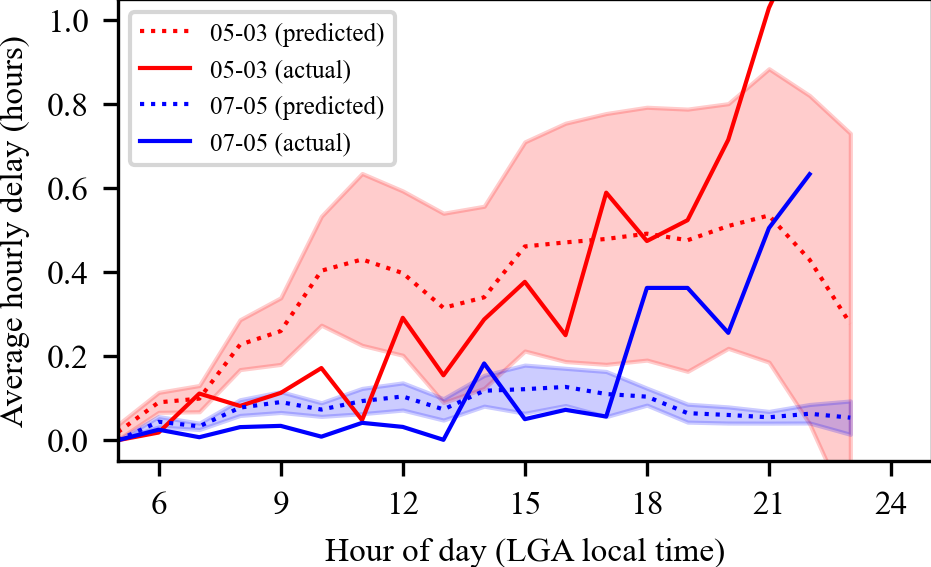
\includegraphics[width=0.7\linewidth]{media/posterior_predictive_comparison_alt.png}
    \caption{Actual and predicted mean hourly delays using our model, with a demand-induced delay applied on one day (red) and nominal operations on the other (blue).}
    \label{fig:pp-comparison-alt}
\end{figure}

% Actual vs predicted hourly delay using our model for two days, the plot in red shown for a day with weather-induced delay that our model successfully replicates (predicted average and standard deviation for 20 samples shown in the plots). The plot in blue shows hourly delays for a day with observed delays to be less than 15 minutes.

Similarly, we examine another pair of days, May 3, 2019 (day 1) and July 5, 2019 (day 2). This time, we have $w_1=(1.609,162.7)$ and $w_2=(10.0,574.9)$, so $d_{w,1}\approx d_{w,2}\approx 1$. However, this time we have $y_1$ above the threshold $\yth$ and $y_2$ below it, so $d_{y,1}=1$ and $d_{y,1}=0$. Similarly to before, we follow the actual observation for comparison, so we use $d_{x,1}=1$ and $d_{x,2}=0$. We visualize this in \cref{fig:pp-comparison-alt}, where we can see the effect of varying the imposed demand in our generative model, and that it also resembles reality for the two day in question.

In these two case studies, we have seen that our learned model and posteriors, although somewhat coarse, do appear to be capable of generating useful and realistic results. Because of the simplified model, we can simply sample adversarial weather conditions by using the learned thresholds, but we will leave investigating more complex structures as part of the plan for future work.

\section{Summary}
\label{sec:atrds-summary}

In this chapter, we developed a guiding case study on weather and delays at LGA. First, we analyzed weather and schedule data along with observed delays to motivate both the choice of weather variables and inclusion of both weather and schedule data, as opposed to just weather data. Then, we developed an amortized variational inference based framework for simultaneously clustering data points into meaningful groups and learning representatives posteriors for each group, and showed via implementation that our learned generative model can produce useful predictive results.